\subsection{Commodity and Commodity Derivatives}

\begin{remark} \hlt{Characteristics of Commodity as an Asset Class}\\
Commodities' value derives from either use as consumables, or as inputs to production of goods and services.\\
As some commodities need to be processed or are perishable, to account for growth and extraction patterns and logistic associated with transportation of these physical goods.\\
Storage costs can lead to forward prices that are higher the further the forward settlement date is in the future.\\
Spot price of commodity can be viewed as discounted value of expected selling price at a future date.\\
Convergence of forward/future to spot is not guaranteed if delivery is required, or market participants do not have ability to make or take delivery of the commodity.
\end{remark}

\begin{remark} \hlt{Fundamental Analysis of Commodities}
\begin{enumerate}[label=\roman*.]
\setlength{\itemsep}{0pt}
\item Direct Announcements: government or private agencies broadcast inventory and production data which can be used to infer demand.
\item Component Analysis: breaking down of high-level supply and demand into various components, with application of stock and flow approach. Stock or potential production sets boundaries on what is actually produced or wanted. Flow considers utilisation of the stock of raw material.\\
Note that a new policy such as stricter emission standards may affect both supply and demand. Political unrest may disrupt consumption.
\item Timing Considerations: seasonality and logistics that may affect demand and supply. 
\item Macroeconomic Factors: inflation may result in an increase in demand for commodities. Low interest rates may increase capital spending and demand for commodities in the medium term.
\end{enumerate}
\end{remark}

\subsubsection{Characteristics of Commodities Sector}

\begin{remark} \hlt{Energy Sector} \\
Fuel transportation, industrial production, electricity generation.\\
Products includes crude oil, natural gas, coal, refined oil products (gasoline, heating oil etc).
\begin{enumerate}[label=\roman*.]
\setlength{\itemsep}{0pt}
\item Stocks: discovery and depletion of new fields, economic and political costs, certainty of access to fields, refinery technology and maintenance, power plant type, construction, economic (GDP) size
\item Flows: pipeline and tanker reliability, seasonality, adverse weather, automobile/truck sales, geopolitical instability, environmental requirements, economic (GDP) growth
\end{enumerate}
\end{remark}

\begin{remark} \hlt{Lifecycle of Energy Sector}
\begin{enumerate}[label=\roman*.]
\setlength{\itemsep}{0pt}
\item Extraction: drilling location selected after surveys. Water may be required to create pressure (fracking)
\item Storage: crude oil is commercially stored for few months, oil may be stored on tanker ships. Natural gas may be delivered directly via pipeline, or injected to storage for winter months before consumption.
\item Refining: crude oil is distilled into component parts with cracking. Distilled products may be consumed.
\end{enumerate}
Crude oil market's most commonly traded contracts are WTI and Brent, representing high-quality refinery input that exploration and production companies can use as a hedging device.\\
Refineries are expensive to build as processing a low grade crude oil requires more investment. Pipeline costs are expensive but pale in comparison with costs and risks of oil exploration.
\end{remark}

\begin{remark} \hlt{Industrial/Base Metals Sector} \\
Materials for durable consumer goods, industry and construction.\\
Products include copper, aluminium, nickel, zinc, lead, tin, and iron.
\begin{enumerate}[label=\roman*.]
\setlength{\itemsep}{0pt}
\item Stocks: mined acreage, smelter capacity, economic (GDP) stage of industrial/consumer development
\item Flows: government industrial and environmental policies, economic (GDP) growth, automobile/truck sales, infrastructure investent
\end{enumerate}
\end{remark}

\begin{remark} \hlt{Precious Metals Sector} \\
Certain metals that act as monetary stores of value (as well as industrial uses).\\
Products include gold, silver, and platinum.
\begin{enumerate}[label=\roman*.]
\setlength{\itemsep}{0pt}
\item Stocks: mined acreage, smelter capacity, fiat money supply/banking development
\item Flows: central bank monetary policy, geopolitics, economic (GDP) growth
\end{enumerate}
\end{remark}

\begin{remark} \hlt{Lifecycle of Industrials and Precious Metals Sector}
\begin{enumerate}[label=\roman*.]
\setlength{\itemsep}{0pt}
\item Extraction: ore (raw earth with $~2\%$ metal content is removed via mine or open pit. Ore is ground into powder and concentrated to $~25\%$ purity.
\item Smelting: purified ore is heated, more impurities removed as slag, increasing metal content to $60\%$. Further processes increase concentration to $99.99\%$.
\item Storage/Logistics: purified metal is held in bonded warehouse until shipment
\end{enumerate}
Economies of scale is crucial; marginal costs decline substantially with both scale and utilisation. Overproduction continues until smaller or financially weaker competitors are forced to shutdown.\\
There is lack of seasonality in production of metals. Variability comes from demand.
\end{remark}

\begin{remark} \hlt{Livestock Sector} \\
Animals raised for human consumption.\\
Products include hogs, cattle, sheep, poultry.
\begin{enumerate}[label=\roman*.]
\setlength{\itemsep}{0pt}
\item Stocks: herd size, processing plant capacity, consumer preferences, feed availability/cost
\item Flows: speed of maturity to slaughter weight, economic (GDP) growth/consumer income, disease, weather
\end{enumerate}
\end{remark}

\begin{remark} \hlt{Lifecycle of Livestock Sector}\\
Good weather and access to high-quality pasture and feed accelerate weight gain, resulting in fluctuation of animals ready for slaughter. Timing to maturity increases with size of livestock.\\
Livestock has a significant seasonal component. Hog and cattle futures may be used to hedge commitments.\\
Grain futures are used to hedge against cost of feeding an animal.
\end{remark}

\begin{remark} \hlt{Gains Sector} \\
Provide human and animal sustenance but may also be distilled into fuel (i.e., ethanol).\\
Products include corn, soy, wheat, and rice.
\begin{enumerate}[label=\roman*.]
\setlength{\itemsep}{0pt}
\item Stocks: arable farmland, storage/port facilities (infrastructure), human and animal population size
\item Flows: weather, disease, consumer preferences, GMO, biofuel substitution, population growth
\end{enumerate}
\end{remark}

\begin{remark} \hlt{Lifecycle of Grains Sector}
\begin{enumerate}[label=\roman*.]
\setlength{\itemsep}{0pt}
\item Planting: placing the seeds in the ground after preparation/fertilisation work
\item Growth: emerging of seedling to full height
\item Pod/Ear/Head Formation: food grain is created by the plant
\item Harvest: collection of grain by the farmer.
\end{enumerate}
As demand is constant, grains are stored in silos and warehouses to maintain stockpiles.\\
Monitoring purchasing patterns of government tenders can provide details on grain demand.\\
Grains futures may be used to hedge exposure, and contract delivery months reflect the growth cycle of grains.
\end{remark}

\begin{remark} \hlt{Softs (Cash Crops) Sector} \\
Crops sold for income and often seen as luxuries.\\
Products include cotton, cocoa, sugar, coffee
\begin{enumerate}[label=\roman*.]
\setlength{\itemsep}{0pt}
\item Stocks: arable farmland, storage/port facilities (infrastructure), economic (GDP) size
\item Flows: weather, disease, consumer prefs, biofuel substitution, economic (GDP) growth/consumer income
\end{enumerate}
\end{remark}

\begin{remark} \hlt{Lifecycle of Softs Sector}\\
Production cycles and storage options vary by product. Coffee is harvested every month, stored in warehouses after transport. Local buyer than roast the beans and ships them to retail location.\\
Robusta are lower quality with lower variety, traded in London. Arabic is the higher quality variant, traded in New York. Futures contracts are for the un-roasted beans.\\
Farmers and distributers sell future contracts to hedge sales price of production, coffee roasters buy futures contracts to hedge coffee bean purchase costs. Contract maturities match product delivery schedules.
\end{remark}

\subsubsection{Valuation of Commodity and Derivatives}

\begin{remark} \hlt{Pricing Terminologies}
\begin{enumerate}[label=\roman*.]
\setlength{\itemsep}{0pt}
\item Spot price: current price to deliver a physical commodity
\item Futures price: price agreed on to deliver or receive a defined quantity at a future date
\item Basis: difference between spot and futures prices.
\item Backwardation: spot price $>$ futures price. Future prices at nearer dates $>$ further dates
\item Contango: futures price $>$ spot price. Future prices at further dates $>$ nearer dates
\item Calendar spread: difference between futures price of nearer maturity and more-distant maturity
\end{enumerate}
Futures market in backwardation results in long futures positions with positive roll return (futures prices $<$ spot prices). Since futures prices converge to spot prices, there is positive return over time.\\
Futures market in contango results in long futures positions with negative roll return. As futures prices converge to spot prices, this results in decrease in value of long futures position.
\end{remark}

\begin{remark} \hlt{Theories of Futures Returns: Insurance Theory by John Keynes}\\
Desire of commodity producers to reduce price risk that drive commodity future returns.\\
Producers hedge price risk by selling futures contracts, driving down futures prices.\\
Future pries $<$ spot price to provide a return to those buying futures. Resulting positiver return to buyers is their return of providing insurance against price uncertainty to producers. Backwardation is hence 'normal'.\\
Empirical evidence shows that buying futures has not resulted in extra returns for providing insurance. Many markets are in contango instead, which imply negative return for providing insurance to producers.
\end{remark}

\begin{figure}[H]
\centering
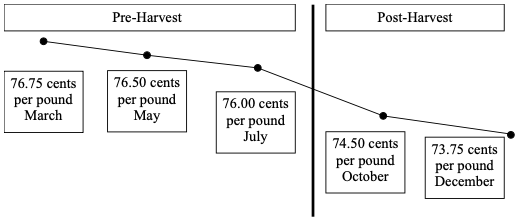
\includegraphics[scale=0.5]{alts/normalbackwardation}
\caption{Normal backwardation}
\end{figure}

\begin{remark} \hlt{Theories of Futures Returns: Hedging Pressure Hypothesis}\\
Insurance Theory with additional hedging behaviour of commodity consumers.\\
Consumers hedging price risk will long future, resulting in more upward price pressure.\\
If producer's hedging behaviour dominates, there will be backwardation. If consumer's hedging pressure dominates, there will be contango. If forces are equal, there will be a flat commodity curve.\\
Producers face more concentrated price risk than consumers, as actual cost of commodity may only represent small proportion of total cost of production or of total income.\\
Both producers and consumers may be speculators in the market. Also, hedging pressure is non-observable.
\end{remark}

\begin{figure}[H]
\centering
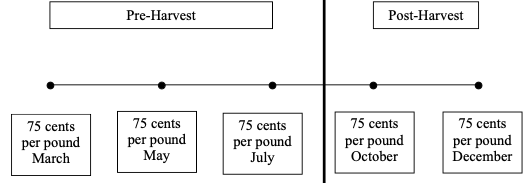
\includegraphics[scale=0.5]{alts/balancedhedging}
\caption{Balanced Hedging of Producers and Consumers}
\end{figure}

\begin{remark} \hlt{Theories of Futures Returns: Theory of Storage}\\
Whether futures market is in backwardation or contango depends on relationship between cost of storage and benefits of holding physical inventory.\\
When costs $>$ benefits, futures are more attractive than current inventory, hence futures price $>$ spot price.\\
When benefits $>$ costs, holding inventory is more attractive, hence spot price $>$ futures price.
\begin{equation}
\text{Futures Price} = \text{Spot Price} + \text{Storage Costs} - \text{Convenience Yield} \nonumber
\end{equation}
\end{remark}

\begin{remark} \hlt{Total Return Components of Commodity Futures}
\begin{enumerate}[label=\roman*.]
\setlength{\itemsep}{0pt}
\item Price Return (Spot Yield): change in spot prices, proxied by futures prices on near-month contracts.
\begin{equation}
\text{Price Return} = \frac{S_{t+1} - S_{t}}{S_{t}} \nonumber
\end{equation}
\item Roll Return (Roll Yield): for maintaining a position over time, where expiring futures position must be closed out and reestablished with new position further in the future. Roll return positive if price curve is in backwardation, and may be negative if price curve is in contango.
\begin{equation}
\text{Roll Yield} = \frac{F_{\text{Expiring}} - F_{\text{New}}}{F_{\text{Expiring}}} \times \text{\% Rolling Futures Positions} \nonumber
\end{equation}
Roll return is modest over multiple periods, but may be significant portion of total return in single period.
\item Collateral Yield: yield for bonds or cash used to maintain futures positions, with an initial margin. 
\end{enumerate}
With an index, return from rebalancing components is also added to total returns.
\end{remark}

\begin{remark} \hlt{Total Return Swap}\\
Swap buyer (long) receive periodic payments based on change in futures price of commodity plus return on collateral, in return for series of fixed payments.\\
Each period, long will receive total return on holding commodity times notional principal amount, net of payment to short. If total return is negative, long makes fixed payment plus negative return on commodity over the period, times the notional amount.\\
Used by institutions to gain exposure to price risk of underlying without holding the commodity or managing a long position in futures contracts over time.
\end{remark}

\begin{remark} \hlt{Excess Return Swap}\\
Party may make single payment at initiation of swap, then receive periodic payments of any percentage by which commodity price exceeds fixed or benchmark value, times notional value of swap.\\
If commodity price does not exceed fixed value, no payments are made.
\end{remark}

\begin{remark} \hlt{Basis Swap}\\
Variable payments based on difference in price of two commodities. One commodity has liquid traded futures available for hedging; the other has no liquid futures contracts. As price changes to two commodities are positively correlated, the difference (basis) between them changes over time.\\
Combining a hedge using liquid futures on basis swap allows hedging of price risk from the input that does not have a liquid futures market.
\end{remark}

\begin{remark} \hlt{Variance Swaps, Volatility Swaps}\\
Underlying factor is volatility of commodity price. If volatility of commodity price is higher than expected level of volatility specified in swap, buyer receives payment; else seller receives payment.\\
A similar swap settles based on variance in price levels of the commodities.
\end{remark}

\begin{remark} \hlt{Commodity Indexes Variations}\\
A commodity index is investable if the index can be replicated with liquid futures contracts.\\
Commodity indexes differ on the following:
\begin{enumerate}[label=\roman*.]
\setlength{\itemsep}{0pt}
\item Mix and weights of constituent commodities, which will result in differences in returns
\item Equal weightage, or weightage by some factor (i.e., value of global production of an individual commodity or commodity sector)
\item Passive strategy by rolling expiring futures into near-month contract each month. Active strategy by maximising roll return, by selecting further-out contracts with greatest backwardation or smallest contango.
\item Frequency of rebalancing, which may capture gains from either mean reversion over shorter periods, or from gains from trend of commodity prices over long term.
\end{enumerate}
\end{remark}